\documentclass[prb,twocolumn,showpacs,preprintnumbers,amsmath,amssymb, superscriptaddress]{revtex4-2}

%\usepackage[magyar]{babel}
%\usepackage[makeroom]{cancel}
\usepackage{amsmath}    % need for subequations
\usepackage{amssymb}
\usepackage{graphicx}   % need for figures
\usepackage{verbatim}   % useful for program listings
\usepackage{color}      % use if color is used in text
%\usepackage{subfigure}  % use for side-by-side figures
\usepackage{hyperref}   % use for hypertext links, including those to external documents and URLs
%\usepackage{blindtext}
\usepackage[normalem]{ulem}
%\usepackage{xpatch}
\usepackage{natbib}
\usepackage{fixmath}
\usepackage{enumitem}
\usepackage{dsfont}
\usepackage{subcaption}

\def \brc #1{\left\lbrace #1 \right\rbrace}
\def \loc {\mathrm{loc}}

% Until we finalize the notation of the total particle number
\newcommand{\n}{N}

\hypersetup{colorlinks,linkcolor=blue,urlcolor=blue,citecolor=blue}
\newcommand{\uv}[1]{\ensuremath{\mathbf{\hat{#1}}}} % for unit vector
\newcommand{\gv}[1]{\ensuremath{\mbox{\boldmath$ #1 $}}} % 
\newcommand{\rem}[1]{  {\color{red} #1}  }
%\newcommand{\g}[1]{{\bf #1 }} %
\newcommand{\beq}{\begin{equation}}
\newcommand{\eeq}{\end{equation}}
\newcommand{\bea}{\begin{eqnarray}}
\newcommand{\eea}{\end{eqnarray}}
\newcommand{\blabel}{\,b}
\newcommand{\alabel}{\,a}
\newcommand{\Lspace}{{\mathit{\mathbb{L}}}}

\newcommand{\bbGamma}{{\mathpalette\makebbGamma\relax}}
\newcommand{\makebbGamma}[2]{%
  \raisebox{\depth}{\scalebox{1}[-1]{$\mathsurround=0pt#1\mathbb{L}$}}%
}

\newcommand{\e}{\text e}
\newcommand{\zp}{\mathbb Z^+}
\newcommand{\z}{\mathbb Z}
\newcommand{\hint}{H_{\text{int}}}
\newcommand{\re}{\text{Re }}
\newcommand{\hc}{\text{h.c.}}
\newcommand{\cc}{\text{c.c.}}
\newcommand{\w}{\omega}
\newcommand{\be}{\begin{equation}}
\newcommand{\ee}{\end{equation}}
\newcommand{\Nedge}{N_{\rm edge}}



\definecolor{darkgreen}{rgb}{0,0.5,0}
\definecolor{orange}{rgb}{1,0.5,0}
\definecolor{grey}{rgb}{.6,.6,.6}
\newcommand{\rc}[1]{\textcolor{red}{#1}}
%\bibliographystyle{apsrev4-1}
%\newcommand{\jav}[1]{#1}
\newcommand{\scrap}[1]{{\color{orange}{\sout{#1}}}}
\newcommand{\cpm}[1]{{\color{blue}{#1}}}

\newcommand{\dr}{\text d^3r}
\newcommand{\dfi}{\text d\varphi}
\newcommand{\dd}{\text d}
\newcommand{\tr}{\tilde r}
\newcommand{\tn}{\tilde n}
\newcommand{\tz}{\tilde z}
\newcommand{\tc}{\tilde c}
\newcommand{\tS}{\tilde S}


\newcommand{\heff}{H_{\text{eff}}}
\newcommand{\hkin}{H_{\text{kin}}}

\newcommand{\pp}{P^{++}+P^{--}}
\newcommand{\ps}{P^{\text(S)}}
\newcommand{\pa}{P^{\text(A)}}
\newcommand{\psn}{P_{S=0}}
\newcommand{\pse}{P_{S=1}}
\newcommand{\eppn}{E^{+}_{0}}
\newcommand{\eppe}{E^{+}_{1}}
\newcommand{\ese}{E^{\text{(S)}}_{1}}
\newcommand{\esn}{E^{\text{(S)}}_{0}}
\newcommand{\eae}{E^{\text{(A)}}_{1}}
\newcommand{\ean}{E^{\text{(A)}}_{0}}
\newcommand{\kent}{k\in\text{NT}}
\newcommand{\meV}{\,{\rm meV}}
\newcommand{\ie}{{\it i.e. }}
\newcommand{\bra}[1]{\langle #1|}
\newcommand{\ket}[1]{|#1\rangle}
\newcommand{\average}[1]{\langle #1\rangle}

%\newcommand{\scrap}[1]{{\color{red}{\sout{#1}}}}


\newcommand{\bK}{\mathbf K}
\newcommand{\bS}{\mathbf S}
\newcommand{\bk}{\mathbf k}
\newcommand{\bq}{\mathbf q}
\newcommand{\ba}{\mathbf a}
\newcommand{\bC}{\mathbf C}
\newcommand{\bH}{\mathbf H}


\newcommand{\bx}{\mathbf x}
\newcommand{\br}{\mathbf r}
\newcommand{\brp}{{\mathbf r}'}
\newcommand{\bxp}{{\mathbf x}'}


\newcommand{\g}{{\gamma}}
\newcommand{\ds}{\displaystyle}
\newcommand{\1}{{1\hspace*{-0.5ex} \textrm{l} \hspace*{0.5ex}}}

\newcommand{\cL}{{\cal L }}
\newcommand{\fL}{\mathfrak{ L }}
\newcommand{\cH}{{\cal H }}
\newcommand{\fH}{\mathfrak{H }}

\newcommand{\cQ}{{\cal Q}}
\newcommand{\cG}{{\cal G}}
\newcommand{\cg}{{\cal g}}
\newcommand{\cS}{{\cal S}}
\newcommand{\cJ}{{\cal J}}
\newcommand{\cN}{{\cal N}}
\newcommand{\chU}{\hat{\cal U}}
\newcommand{\hU}{{\hat U}}

\newcommand{\ketL}[1]{|#1 )}
\newcommand{\braL}[1]{( #1|}
\newcommand{\averageL}[1]{( #1 )}
\newcommand{\tsigma}{{\tilde \sigma}}

\def\doubleunderline#1{\underline{\underline{#1}}}

\newcommand{\mk}[1]{{\color{blue} #1}}


\newcommand{\tp}[1]{{\color{darkgreen} #1}}

\begin{document}
\title{Theoretical modeling of the collective tunneling of a Wigner necklace}
\author{Dominik  Szombathy}
\affiliation{Department of Theoretical Physics,  Institute of Physics, Budapest University of Technology and Economics,  Budafoki \'ut 8., H-1111 Budapest, Hungary}
\affiliation{MTA-BME Quantum Dynamics and Correlations Research Group, 
Institute of Physics, Budapest University of Technology and Economics,  Budafoki \'ut 8., H-1111 Budapest, Hungary}
\author{Mikl\'os Antal Werner}
\affiliation{Department of Theoretical Physics,  Institute of Physics, Budapest University of Technology and Economics,  Budafoki \'ut 8., H-1111 Budapest, Hungary}
\affiliation{MTA-BME Quantum Dynamics and Correlations Research Group, 
Institute of Physics, Budapest University of Technology and Economics,  Budafoki \'ut 8., H-1111 Budapest, Hungary}
\author{C\u at\u alin Pa\c scu Moca}
\affiliation{Department of Theoretical Physics, Institute of Physics, Budapest University of Technology and Economics, Budafoki \'ut 8., H-1111 Budapest, Hungary}
\affiliation{Department of Physics, University of Oradea,  410087, Oradea, Romania}
\author{Gergely Zar\'and}
\affiliation{Department of Theoretical Physics,  Institute of Physics, Budapest University of Technology and Economics,  Budafoki \'ut 8., H-1111 Budapest, Hungary}
\affiliation{MTA-BME Quantum Dynamics and Correlations Research Group, 
Institute of Physics, Budapest University of Technology and Economics,  Budafoki \'ut 8., H-1111 Budapest, Hungary}
%\affiliation{ BME-MTA Exotic Quantum Phases Group, Institute of Physics, 
%Budapest University of Technology and Economics, H-1111 Budapest, Hungary}
\date{\today}
\begin{abstract}
To be written. 
\end{abstract}
\maketitle

\section{Introduction}
\begin{itemize}
\item Nanotube description
\item Experimental background
\item Wigner Crystal and $r_s$ values in this system
\end{itemize}

\begin{figure}[h!]
    \begin{center}
     \includegraphics[width=0.7\columnwidth]{Experimental_Setup.png}
     \vskip 10pt
     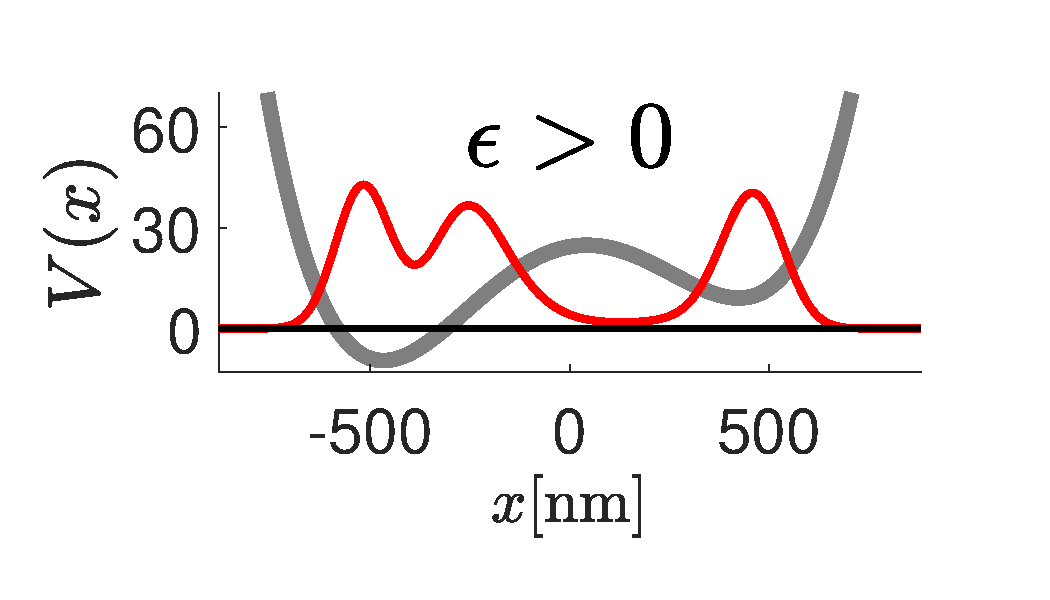
\includegraphics[width=0.49\columnwidth]{Fig_WaveFunction_Potential_NegEps_v1}
     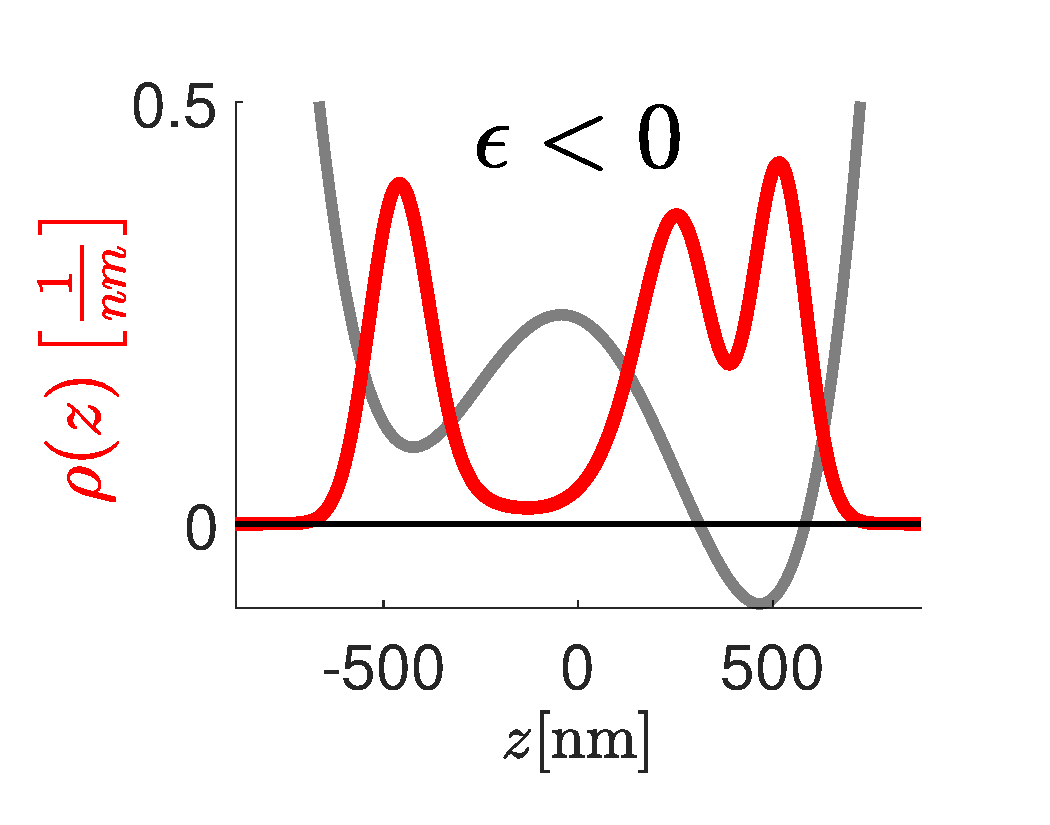
\includegraphics[width=0.49\columnwidth]{Fig_WaveFunction_Potential_PosEps}
    \end{center}
    \caption{Top: Sketch of  the experimental setup used to measure the
	 collective tunneling. The gates  
	 $V_{gi}$ are used to shape the double well potential. 
	 The lefthand side of the nanotube is used as a charge detector. 
	 Bottom: Ground state charge densities  (red) obtained via exact diagonlization  for a the double well potential (grey) with 3 electrons, in the case of finite detuning, $\epsilon = \pm 0.1 {\rm{ V/nm}}$, $\eta = 20$ dimensionless interaction parameter, see \eqref{dimless_interaction_param}. eq, plotted using the $l_d = 160 {\rm{ nm}}$ lengthscale.}
     \label{fig:experimental_setup}
\end{figure}
  
 \begin{figure}[h!]
    \begin{center}
    	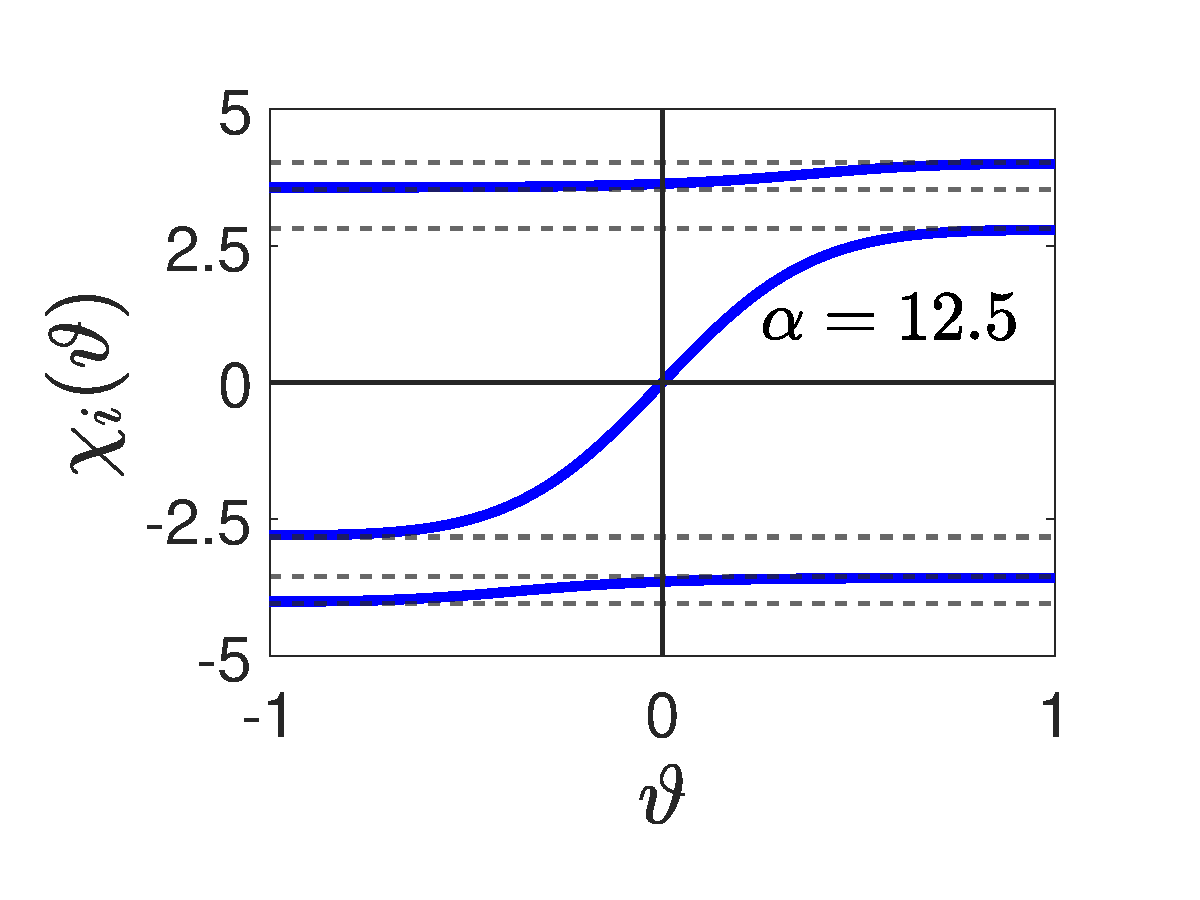
\includegraphics[width=0.8\columnwidth]{Fig_3Particle_Trajectory}
     	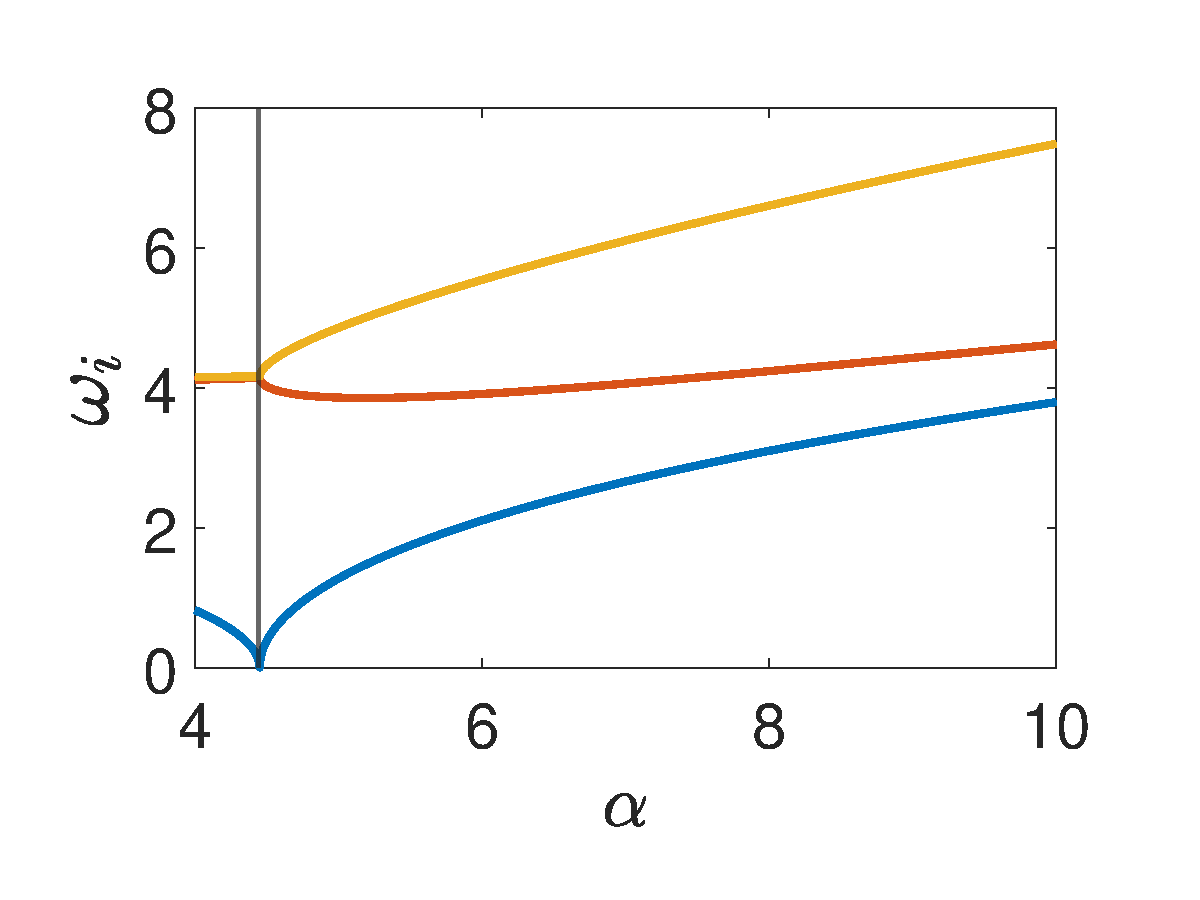
\includegraphics[width=0.8\columnwidth]{Fig_Freqs.pdf}
		
     \caption{Top: Three particle imaginary time trajectories (blue) in the dimensionless units for a specific confinement parameter $\alpha = 12.5$ and $\eta = 20$. Dashed lines show the classical equilibrium positions or instanton turning points for the 3 particles. Bottom: Eigenfrequencies as a function of $\alpha$, for three particles. The vertical line at $\alpha_{cr} \approx 4.45$ marks the beginning of the tunneling regime. For $\alpha > \alpha_{cr}$ two stable positions exist, and the particles move between these by collective tunneling.}
     \label{fig:traj}
    \end{center}
\end{figure}  

\begin{figure*}[h!]
    \begin{center}
    	\begin{tabular}{cc}
    		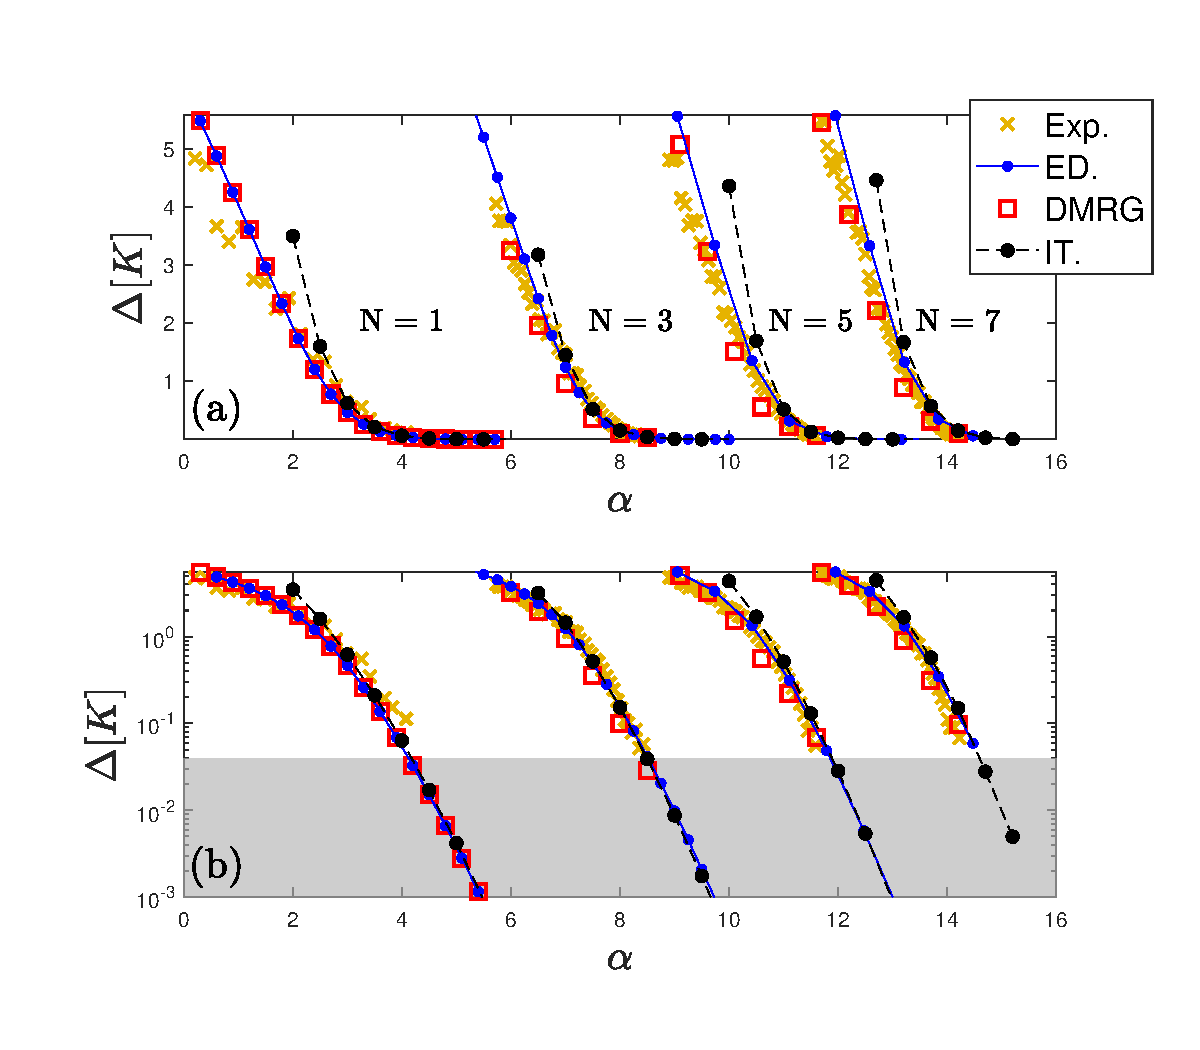
\includegraphics[width=1\columnwidth]{Fig_spectral_gap_exp_fitted_2}
     		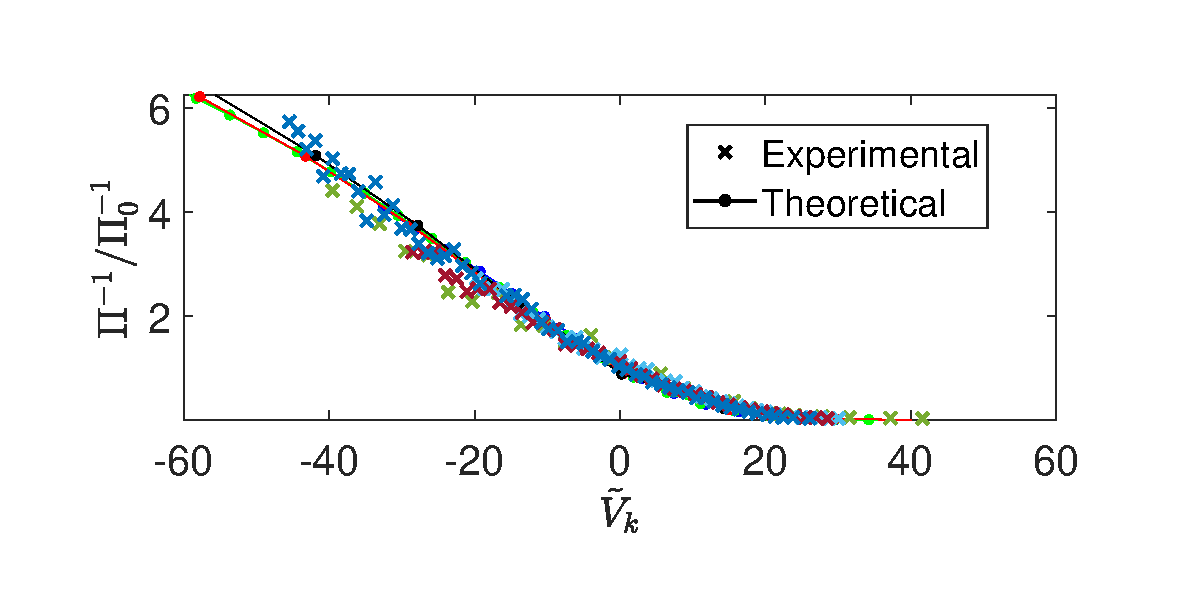
\includegraphics[width=1\columnwidth]{Fig_spectral_gap_exp_log_lin_shahal_scaling_log}
    	\end{tabular}
    	


		 	\caption{(a) and (b) Scaled experimental data for the measured polarization and numerical data for the tunnel splitting using various approaches as function the confinement parameter $\alpha$ that controls the hight of the barrier between the wells. Different curves correspond to different number of electrons in the system. (c) Perpendicular tunneling renormalization factor $R_0$ calculated from the instanton theory. (d) Demonstraition of the universal scaling between the experimental data and the exact diagonalization calculation. Gate voltage $V_k$ adjusts the potential barrier, and $\Pi_0^{-1}$ is a normalization factor obtained from the experimental curves critical $V_k$ value. (I kept it in it's original form from Shahal's ppt) }
     
     \label{fig:experimental_setup}
    \end{center}
\end{figure*}    
  	

\section{Numerical approaches}
\begin{itemize}
\item Effective Hami
\item alpha values; epsilon values
\item what we calculate, trajectories, tunnel splitting, polarization
\end{itemize}

\begin{equation}\label{dimfull_Hamiltonian}
H = \sum_{i = 1}^\n \left[ -\frac{\hbar^2}{2m}\frac{\partial^2}{\partial z_i^2} + \frac{a}{2} z_i^2 + \frac{b}{4}z_i^4 + {c} z_i  \right] + \sum_{i<j}^\n \frac{e^2}{4 \pi \varepsilon_0}\frac{1}{\left| z_i - z_j  \right|}
\end{equation}










\begin{align}
{\text{"Universal scaling"}}\\
v &= (V - \delta V_{\n})/V_\n \\
\tilde{\Delta} &= \Delta\, f_\Delta \\
\tilde{\alpha} &= (\alpha - \alpha_0^{(\n)}) f_{\alpha, \n} \\
{\text{Scaling to }} \alpha \\
\alpha(V) &= \delta\alpha_\n + \frac{1}{V_0} \left(V - \delta V_\n  \right)
\end{align}

\begin{table}[h!]
\begin{tabular}{|c|c|c|c|c|}
\hline
$\n$ & $f_\alpha$   & $\delta V_\n$ [mV] & $V_\n$ [mV]  & $\alpha_0$ \\ \hline
1 & 14.8  & 109  & 1    & 2.2     \\ \hline
3 & 18.5  & 280  & 0.25 & 6.9     \\ \hline
5 & 21.28 & 560  & 0.15 & 10.4    \\ \hline
7 & 22.2  & 850  & 0.13 & 13.2    \\ \hline
\end{tabular}
\end{table}
\subsection{general framework vagy Model(l)ing}\label{SubSect_Framework}
Using the measured experimental potential without the tunneling barrier ($a = 0$) and fitting it with a fourth-order polynomial, the natural length scale of the physical setup can be extracted as:

\begin{equation}
	l_d = \left( \frac{\hbar^2}{m^* \beta} \right)^{1/6} \approx 160 \,{\rm{ [nm]}}.
\end{equation}
Utilizing this natural length scale, the corresponding energy units for such potential can be expressed as:
\begin{equation}
	E_0 = \frac{\hbar^2}{m^* l_d^2} \approx 0.48 \,{\rm{ [meV]}} \approx 5.56 {\rm{ [K]}},
\end{equation}
where $m^*$ represents the effective mass of the charge carriers on the nanotube, thereby making the coefficient of the kinetic part $1/2$. The dimensionless Hamiltonian $\tilde{H} = H/E_0$ then takes the following form:
\begin{equation}\label{dimless_Hamiltonian}
 	\tilde{H} = \sum_{i = 1}^\n \left[ -\frac{1}{2}\frac{\partial^2}{\partial \chi_i^2} - \frac{\alpha}{2}\chi_i^2 + \frac{1}{4} \chi_i^4 + \epsilon \chi_i \right] + \eta \sum_{i < j}^\n \frac{1}{\left| \chi_i - \chi_j  \right|},
\end{equation}
where $\chi_i = z_i/l_d$ is the dimensionless length unit. Additionally, $\eta$ represents the dimensionless interaction strength, while $\alpha$, an analogous parameter to $a$ in \eqref{dimfull_Hamiltonian}.equation, sets the potential barrier height, and $\epsilon$ represents the dimensionless electric field. The dimensionless interaction parameter $\eta$ can be expressed as the ratio of the effective Bohr radius and the length scale:
\begin{equation}\label{dimless_interaction_param}
	\eta = \frac{l_d}{a_B} \approx 20,
\end{equation}
which indicates that this parameter describes this specific nanotube. The fact that $\eta$ is much larger than one suggests that the interaction between the charge carriers is strong.

In the quantum mechanical description, each electron, apart from its coordinate along the nanotube, can be further characterized by its respective spin and valley spin. These properties are omitted in this calculation, as the experimentally available temperature range far exceeds the exchange interaction energy scales.

\subsection{Instanton}\label{SubSect_Instanton}
Feynman's path integral formalism provides valuable insights into quantum tunneling phenomena. This approach describes the time evolution of a quantum system using the time evolution operator for infinitesimally small time steps, rather than solving the Schrödinger equation. In time-independent Hamiltonians, the time evolution operator can be expressed by exponentializing the Hamiltonian. An approximation of the time evolution operator is usually necessary, with one of the most well-known approximations being the Suzuki-Trotter formula [S-T approx; Fenyman]. This formula allows for the decomposition of the time evolution operator into simpler operators, which can be expressed as the exponential of the sum of the Hamiltonian at different times. The propagator can then be expressed as the classical action integrated over the time domain. While only quadratic Hamiltonians are solvable exactly using Feynman's path integral formalism, it can still be extremely useful in cases where the systems description is heavily dependent on the classical behaviour, but where quantum fluctuations can still play an important role in determining its properties.

The effectively one-dimensional tunneling occurs between the classical equilibrium positions of the charge carriers. In the case of a generic quartic potential with paramters $\alpha$ and $\eta$, these positions correpsond to configurations of the Wigner-crystal. The determination of these configurations was accomplished through the use of the Nelder-Mead minimization algorithm and simulated annealing methods [N-M alg.; SA]. The $N$-particle quartic potential together with the interaction term can be represented as follows:
\begin{equation}
	v_\n(\{\chi_i\}_{i=1}^\n) = \sum_{i=1}^\n \left(-\frac{\alpha}{2} \chi_i^2 + \frac{1}{4} \chi_i^4   \right) + \eta \sum_{i < j}^\n \frac{1}{|\chi_i - \chi_j |}.
\end{equation} 
Using $v_\n(\{\chi_i\}_{i=1}^\n)$ we can write the propagator between the latter equilibrium positions as:
\begin{equation}
K(\mathbold{\chi}_0^\prime, \mathbold{\chi}_0, \tilde{T}) = \langle \mathbold{\chi}_0^\prime \vert \e^{-i\tilde{H}\tilde{t}} \vert \mathbold{\chi}_0 \rangle
\end{equation}
where $\mathbold{\chi}_0$ denotes the equilibrium positions, $\tilde{t} = E_0 t/\hbar$ dimensionless time. In the saddle-point approximation the propagator can be brought to a form that spearates the classical action, from the fluctuations around it
\begin{align}
	K(\mathbold{\chi}_0^\prime, \mathbold{\chi}_0, \tilde{T}) =\\
	 e^{iS_{cl}} \int\limits_{\mathbf{r}(0) = 0}^{\mathbf{r}(\tilde{T}) = 0} \mathcal{D}\textbf{r} \exp \left\lbrace  \frac{i}{2} \int_{0}^{\tilde{T}} {\rm{d}} \tilde{t}\, \mathbold{r}(\tilde{t}) \left[ \partial^2_{\tilde{t}} \right. \right.\\
	\left. \left. + \partial^2 v_\n(\mathbold{\chi_{cl}}(\tilde{t}) \right] \mathbold{r}(\tilde{t})\right\rbrace.
\end{align} 
$S_{cl}$ gives the calssical action with the corresponding $\mathbold{\chi}_{cl}$ classical trajectory, $\mathbold{r}(\tilde{t}) = \mathbold{\chi}_{cl}(\tilde{t}) - \mathbold{\chi}(\tilde{t}) $ is the deviation from the calssical path.

Given the equilibrium positions, by the Wick-rotation of time from the dimensionless $E_0 t /\hbar = \tilde{t}$ to $-i\tau$, the imaginary-time classical trajectories can be obtained for a given potential. This is necessary because the height of the tunneling barrier far exceeds the energy of the particles, thus there is no real valued classical trajectory can be obtained. As a result of the Wick-rotation, the action transformes to the Euclidean action as $iS \rightarrow -S_E$, whcich is a function of imaginary time. The Euclidean action can be expressed as:
\begin{equation}\label{ImagAction}
	S_E = S_0 \sum_{i = 1}^\n \int {\rm{d}} \tau \left\lbrace \frac{1}{2}\left( \frac{{\rm{d}} \chi_i}{{\rm{d}} \tau} \right)^2 + v_\n(\{\chi_i\}_{i=1}^\n)   \right\rbrace,
\end{equation}
where $S_0 = (l_d / E_0)^{3/2}$ {\color{red} double check this!!!} gives the units of the action.

The extremal trajectory that minimalizes the action corresponds to a motion between times $t = -\infty$ and $t = \infty$. Motivated by the fact, that the tunneling occurs between the anitsymmetrical, equilibrium particle configurations of the Wigner crystal. To make the calculation of the action more numerically accessible, a further transformation of the time variable is often applied, such as $\vartheta = \tanh\left( {\tau}/{\varrho} \right)$, where $\varrho$ is a tunable paramter of this transformation. The Euclidean action can be expressed as:
\begin{align}\label{FinalAction}
S_E = S_0 \sum_{i = 1}^\n \int\limits_{-1}^{1} {\rm{d}}\vartheta &\left\lbrace \frac{(1 - \vartheta^2)}{2\varrho} \left( \frac{{\rm{d}}\chi_i}{{\rm{d}}\vartheta} \right)^2 \right.\\ \nonumber
&+ \left. \frac{\varrho}{1 - \vartheta^2} v_\n(\{\chi_i\}_{i=1}^\n) \right\rbrace.
\end{align}
While it is possible to perform analytical calculations to determine the trajectory of a single particle, when dealing with a system containing more than two particles ($N \geq 2$), it becomes necessary to employ simulated annealing methods to obtain results.

Despite \eqref{FinalAction}.eqaution shows divergent behaviour at the boundary of the integration domain, it is evident that the displacement of the quartic potential, such that the equilirium configuration's energy is zero, leads to the vanishing of the divergencies. Furthermore, as a known initial condition, the actions kinetic part vanishes exponentially at the boundaries.

Given that the propagator yields equivalent probabilities to both the instanton (left-to-right tunneling) and anti-instanton (right-to-left tunneling) solutions of the Hamiltonian, one may impose symmetry constraints on the particle trajectories. Specifically, one may allow the middle particle's trajectory to evolve freely during the simulated annealing process between $\vartheta=-1$ and the time at which it reaches the midpoint of the potential barriers. Subsequently, one may apply the condition $\chi_{\rm{middle}}(\vartheta)=-\chi_{\rm{middle}}(-\vartheta)$ to ensure symmetry. Similar constraints may be applied to the trajectories of other particles by enforcing $\chi_{i}(\vartheta)=-\chi_{n-i}(-\vartheta)$. Furthermore the time corresponding to reaching the middle point of the potential can be also fixed as $\chi_{\rm{middle}}(\vartheta_0) = 0$ at $\vartheta_0 = 0$, without which the simulated annealing produces unreliable trajectories. For such trajectories see \ref{fig:traj}.top figure. An additional advantageous approach is to contemplate the non-interacting solution to the \eqref{FinalAction} equation (with the interacting equilibrium configuration as boundary condition) as a viable approximation of the particle trajectories. By leveraging these analytical paths as a starting point of the simulated annealing, computational efficiency can be enhanced.\\

Based on the principles of instanton theory [Coleman] and the semiclassical calculations done by [Milnikov], the imaginary-time propagator can be approximated as a product of two terms in the saddle-point approximation for multi-dimensional cases. The first and second term depends only on the imaginary-time classical trajectories, while the rest represents the quantum fluctuations around it. The equation for the propagator is given by:

\begin{align}
K(\mathbold{\chi}_0^\prime, \mathbold{\chi}_0) &= \e^{-S_E} \sqrt{ \frac{2S_E}{\pi}} \left[ \frac{det^\prime \left(-\partial_\vartheta^2 + V^{\prime \prime}_0 (\vartheta))   \right)}{det\left(-\partial_\vartheta^2 + \omega^2_N   \right)}  \right]^{-1/2}\\ \nonumber
&\times \left[  \frac{det^\prime \left(-\partial_\vartheta^2 {\bf{1}} + {\bf{\Omega}}^2 (\vartheta)   \right)}{det\left(-\partial_\vartheta^2 {\bf{1}}+ {\bf{\Omega}}^2_0   \right)}   \right]^{-1/2},
\end{align}
where $\omega_N$ represents the frequency of the softest vibrational mode in the equilibrium configuration with $\n$ particles [see \ref{fig:traj}.bottom figure], and ${\bf{\Omega}}_0$ represents the eigenfrequencies of the equilibrium state. ${\bf{\Omega}}(\vartheta)$ is an $\n - 1$ dimensional matrix computed using the vibrational eigenvectors along the double well potential and the potential shape. The term $det^\prime$ denotes the functional determinant, without including the lowest, zero eigenvalue. This zero eigenvalue corresponds to an arbitrary time shift in the classical trajectories [Schulman].

To determine the value of the second determinant formula, one can introduce Jacobian fields [jac-field] and solve a set of differential equations. An essential aspect of this calculation is the introduction of a coordinate basis transformation on the $\n$ dimensional trajectory. The new basis consists of one parallel and $\n-1$ perpendicular unit vectors with respect to the trajectory, as opposed to $\n$ coordinates that describe the independent particles. It is found that the trajectory's direction is parallel to the eigenvector of the softest vibrational eigenmode.

In this description the trajectory and subsequent calculations can be simplified to an arc-length parametrized effectively one-dimensional description, which takes place in the effective potential, that is created by the collective motion of particles as in \ref{fig:effpot_perpfact}. top figure. This picture makes it possible to express $\mathbold{\Omega}$ by the curvitare of the trajectory parametrized either by imaginary time or arc-length, although the two descriptions yield the same results. Solving numerically the set of differential equations ${\bf{\dot{\Xi}}} = \varrho /(1 - \vartheta^2)\left({\bf{\Omega}^2}(\vartheta) - {\bf{\Xi}}^2(\vartheta)\right)$ with the appropriate boundary conditions that states, that indeed for times close to $\vartheta = \pm 1$ the particles behave like a collective harmonic oscillator.

The previously introduced time scaling parameter $\varrho$ plays an important role in this calculation. It governs the numerical time step sizes across times $\vartheta = \pm 1$. A lower value of $\varrho$ increases the numerical accuracy in the tunneling region at a set resolution, while increasing its value will make the trajectories' beginnings and endings smoother. Although the tunnel splitting's most significant contribution comes from times around $\vartheta_0$, to make numerically accurate calculations, it is necessary to ensure that the trajectories show exponential decay in their derivatives.

In the end the tunnel splitting can be expressed as:

\begin{equation}
\Delta = R_0 \sqrt{\frac{4\omega_\n}{\pi}} P\left[ \mathbold{\chi}(\vartheta) \right] e^{-S_E}.
\end{equation}
where $R_0$ is the renomralization factor coming from the quantum fluctuations around the classical path [see \ref{fig:effpot_perpfact}.bottom figure], $P\left[ \mathbold{\chi}(\vartheta) \right]$ is a momentum-like quantity that depends on the specific trajectory.


\begin{itemize}
\item {\color{red} Dont know where to put this: Note that the real time trajectories are expressable by analytic continuation.}
\item Should I mention the results here, or it will be referenced later in the results section?
\end{itemize}
\begin{figure}[h!]
		\begin{center}
			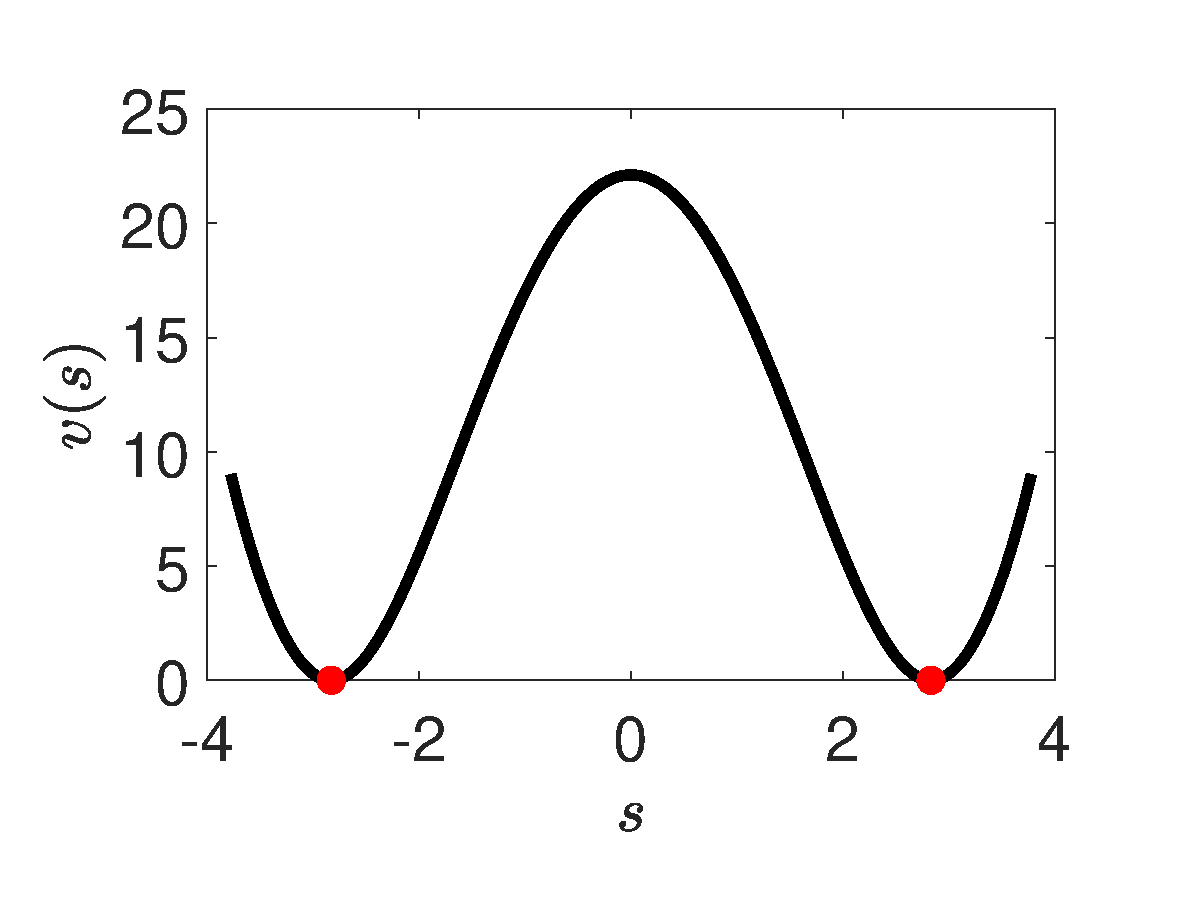
\includegraphics[width=0.9\columnwidth]{SupMatFig_EffectivePotential.pdf}
			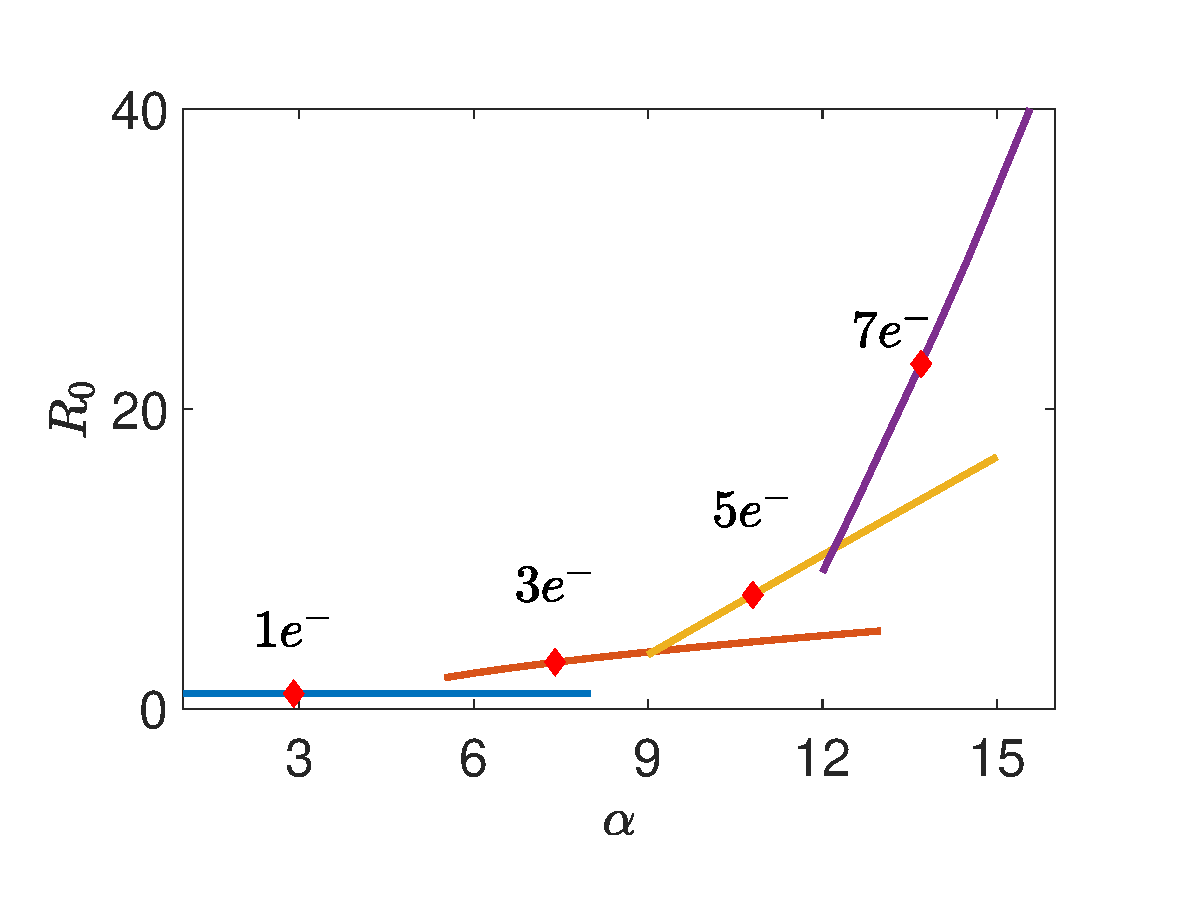
\includegraphics[width=0.9\columnwidth]{Fig_perpfactors.pdf}
			\caption{Top: Effective one-dimensional potential $v(s)$ for $N = 3$ particles, with $ds^2 = \sum_i d\chi_i^2$, for the arc length along the instanton trajectory for $\alpha = 10.5$ and $\eta = 20$. Red dots mark the classical turning points for the tunneling. Bottom: Perpendicular tunneling factors for $\n = 1, 3, 5, 7$. Diamond shapes mark the beginning of the quantum tunneling regime. }
						\label{fig:effpot_perpfact}		
		\end{center}
	\end{figure}
\subsection{Exact diagonalization}
The tunnel splitting can be also investigated using exact diagonalization methods. Considering the dimensionless hamitlonian \eqref{dimless_Hamiltonian}, the state space is the discretized $\mathbold{\chi}(\vartheta)$ space.  A finite-difference method Hamiltonian is then constructed and used to determine the ground state and first excited state's energy, as well as the corresponding "bonding" and "anti-bonding" wavefunction solutions. The tunnel splitting is calculated as the difference between the two energies.However, when the system contains more than one particle and their state space is considered to be equal, the efficient discretization of space becomes a challenge, as the dimension of the finite-difference Hamiltonian increases to its square. The most important condition is that the obtained wavefunction should decay exponentially at therespective state space boundary. 

In the Wigner crystal, the electrons become locaized and thus the describpiton of the i-th elcectron wavefunction does not extend over the whole state space, enabling us to confine the state space for select electrons within the crystal. Utilizing this confinement, we have constructed a Hamiltonian for $N$ particles and calculated the necessary energy levels for the tunnel splitting. we have observed that electrons situated farther from the potential barrier undergo less motion during collective motion compared to electrons closer to it, enabling us to represent their wavefunctions using fewer state space points while keeping the spatial resolution equivalent. The boundaries of each state space can be determined by expanding upon the equilibrium positions in the potential, until the boundary conditions are satsified.





\subsection{DMRG}
\begin{itemize}
\item Basis used
\item I guess technical description here is not that important, myabe in the SUpMat
\end{itemize}


\section{Results}
\subsection{Tunnel Splitting}

\subsection{Charge distribution and polarization}

\begin{equation}
\rho(\mathbold{\chi}) = \bra{\Psi} \sum_{i=1}^\n \delta(\mathbold{\chi} - \mathbold{\chi}_i)\ket{\Psi}
\end{equation}

\begin{equation}
\tilde{P} = \int\limits_{-\infty}^{\infty} {\rm{d}}\mathbold{\chi} \rho(\mathbold{\chi}) \mathbold{\chi}
\end{equation}

\begin{equation}
\rho(\chi) = \sum_{i=1}^n \Psi^\star_i (\chi) \Psi_i(\chi)
\end{equation}

\begin{figure}[h!]
    \begin{center}
     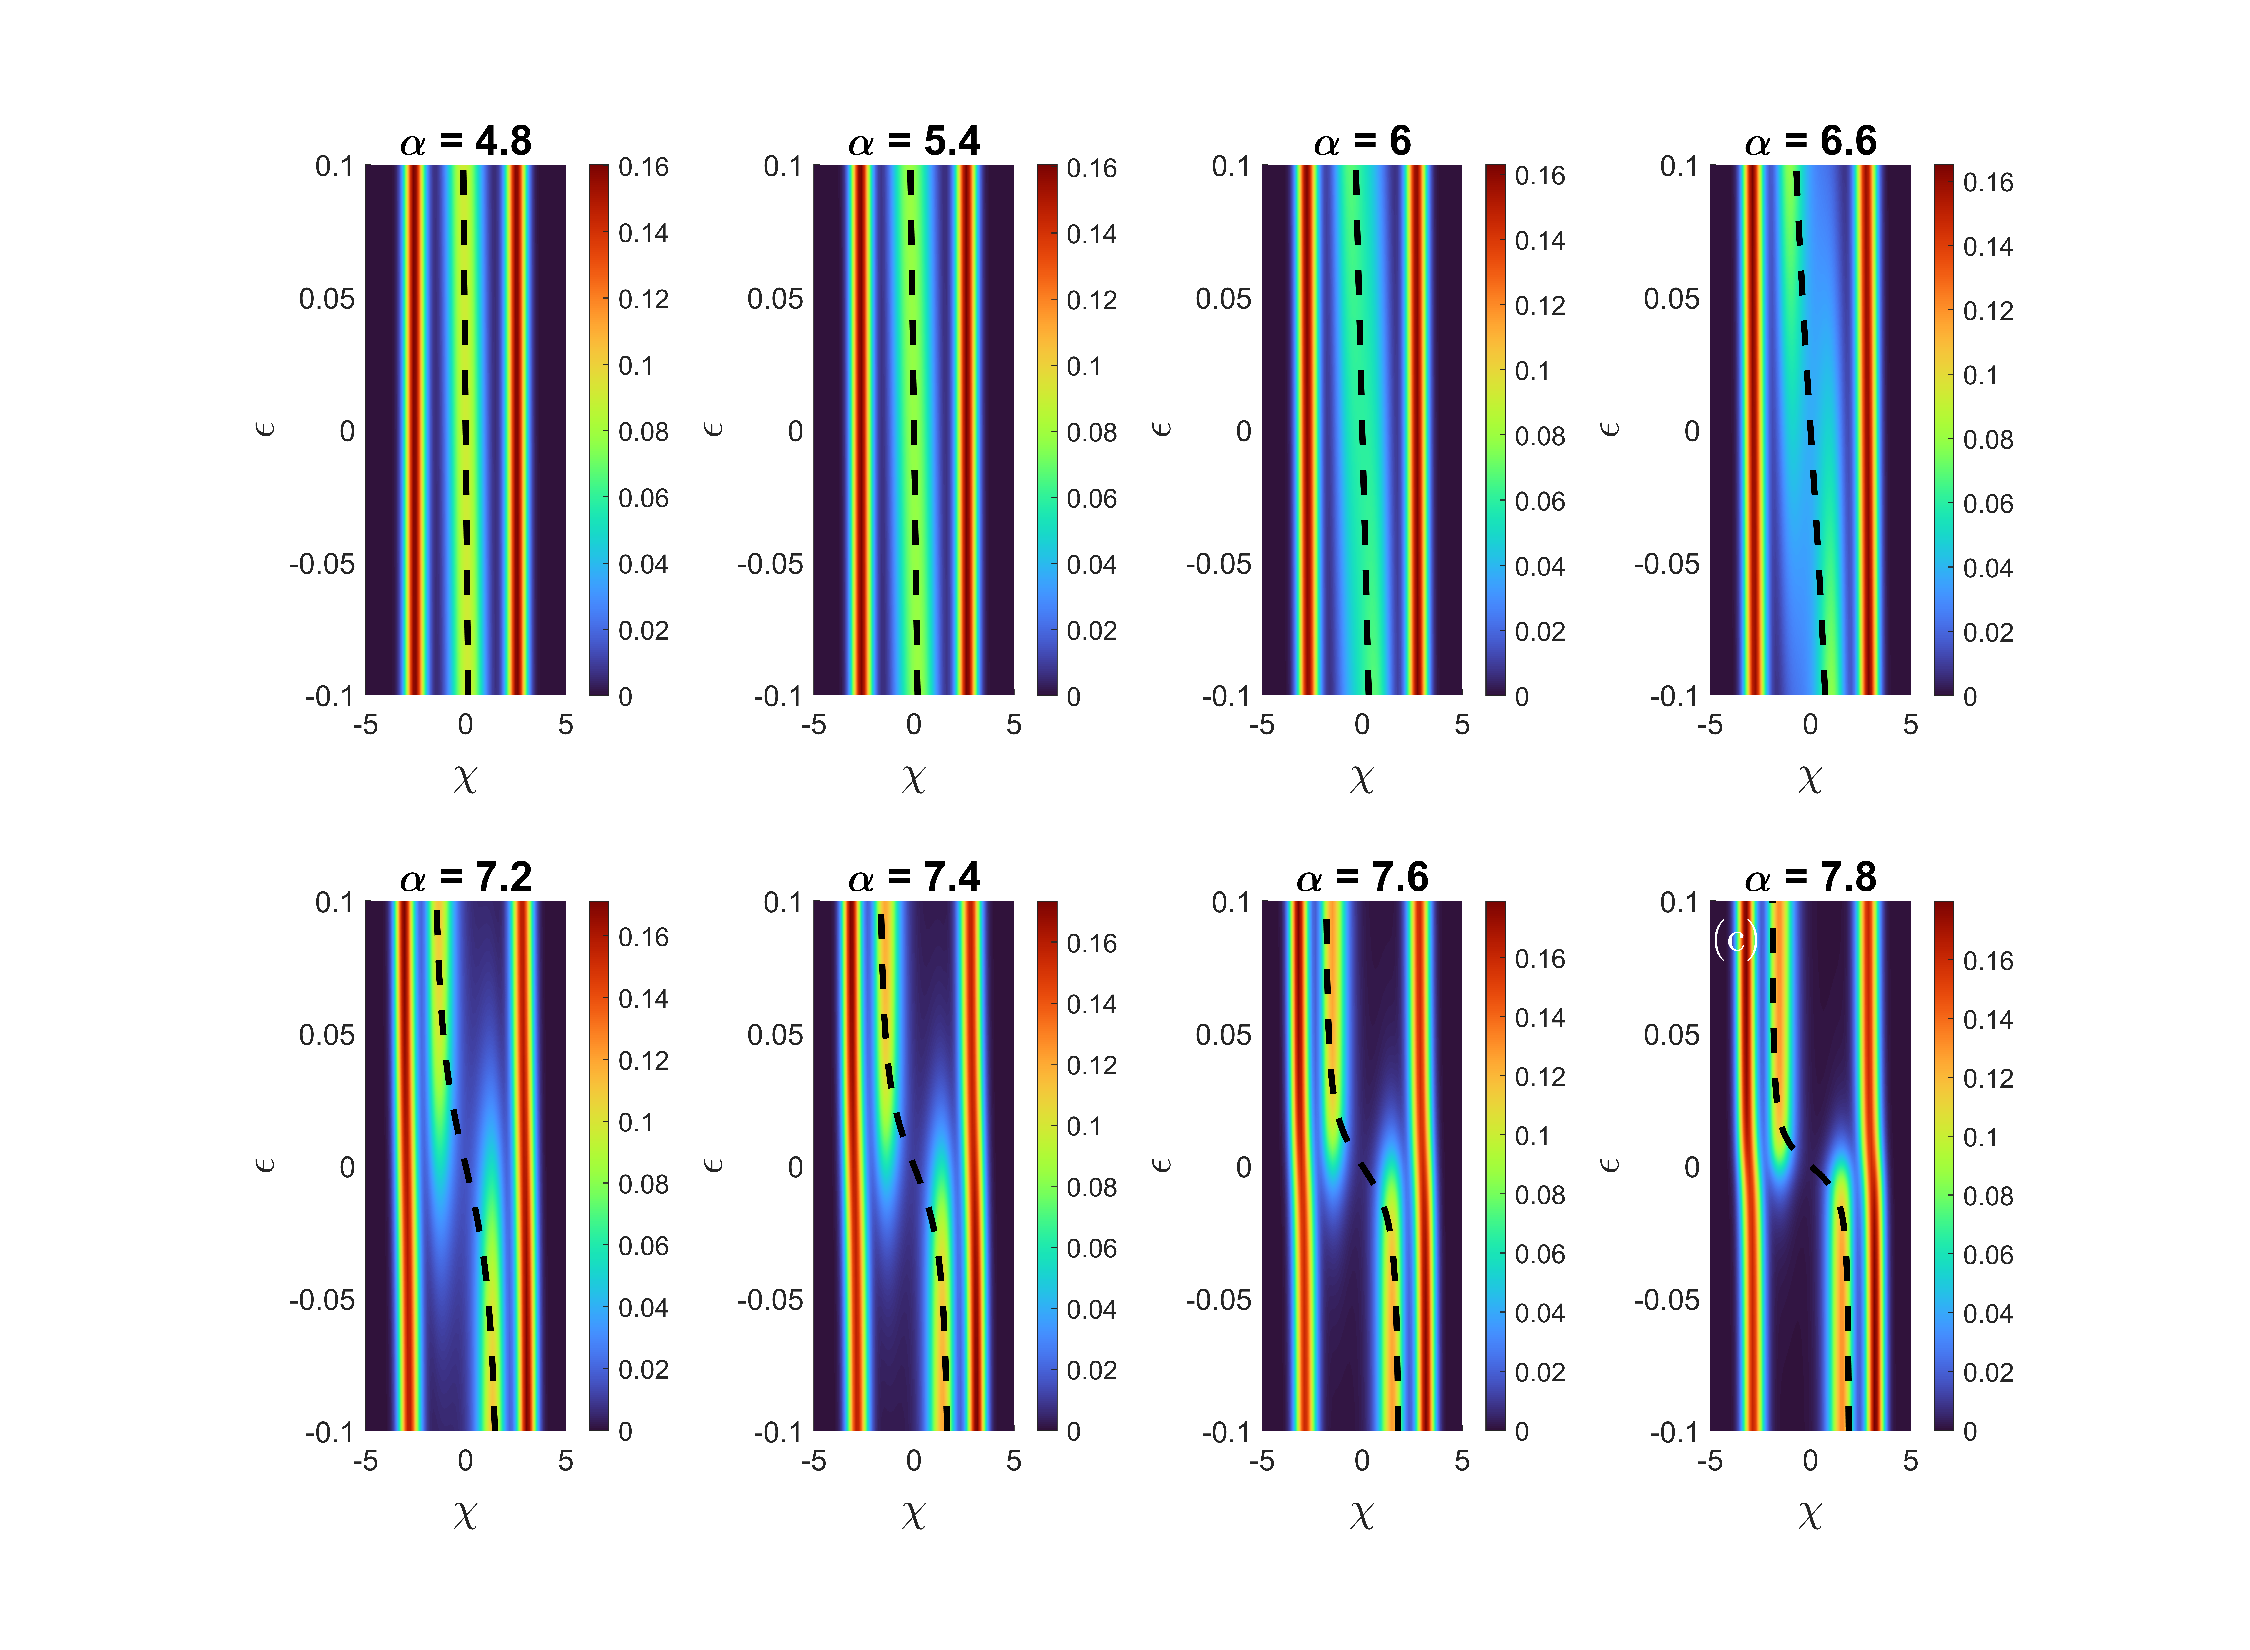
\includegraphics[width=2\columnwidth]{SupMatFig_DensitySeries}
     \label{fig:experimental_setup}
     \caption{Polarization series for $N = 3$ particles. The classical critical point is at $\alpha_{cl}^{N=3} \approx 4.45$, but tunneling occurs above $\alpha = 6$.}
     
    \end{center}
     \end{figure}

\begin{figure}[h!]
	\begin{center}
		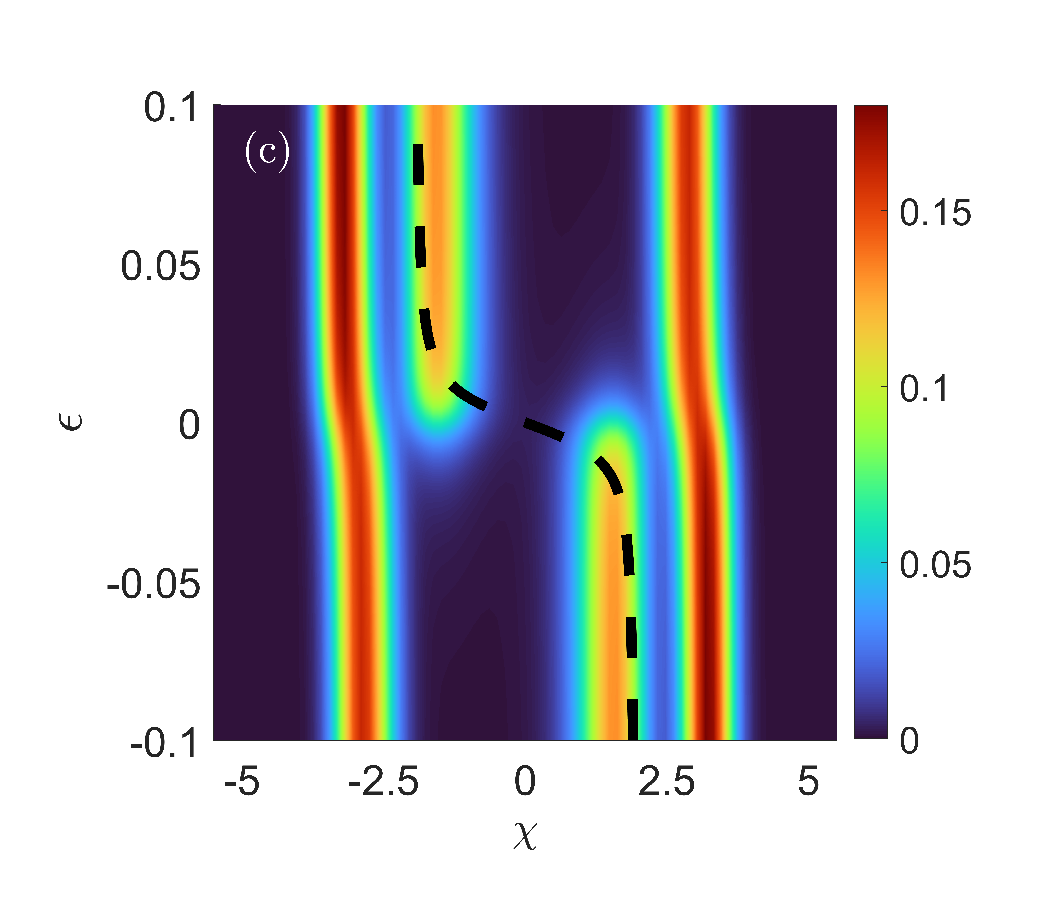
\includegraphics[width=1\columnwidth]{Fig_Polarization_2D}
		
		\caption{Top: Charge density as a function of the dimensionless electric field $\epsilon$ at $\alpha = 7.8$ and $\eta = 20$. The dashed line denotes the polarization in the system.}
	\end{center}
\end{figure}


\begin{figure}
	\begin{center}
	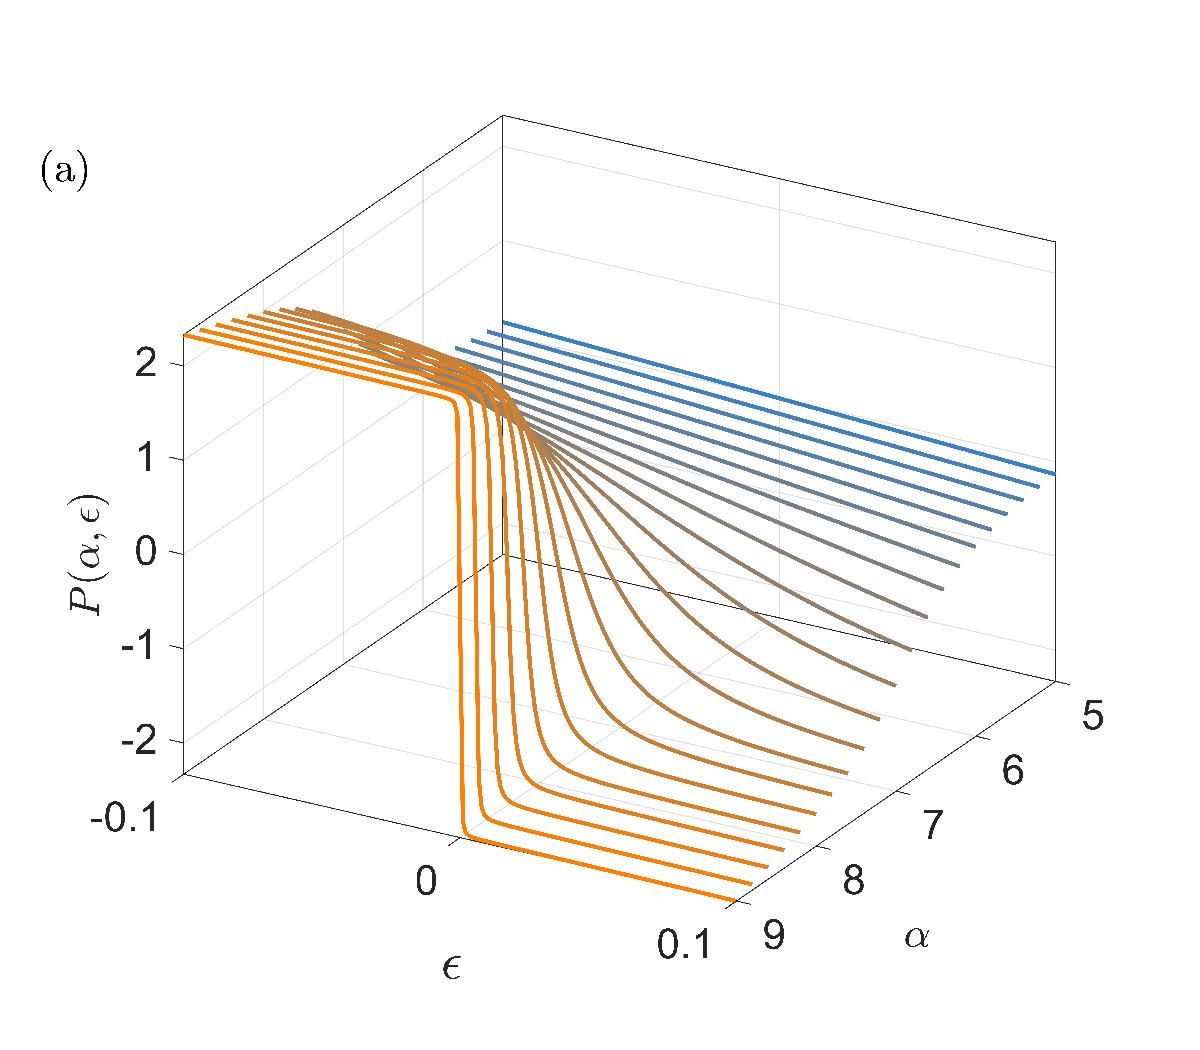
\includegraphics[width=1\columnwidth]{Fig_Polarization_3D_theor}
	\includegraphics[width=1\columnwidth]{Fig_Polarization_3D_exp}
     \caption{Top: Polarization as a function of $\alpha$ and $\epsilon$ as computed by exact diagonalization. Bottom:}
	\end{center}
\end{figure}


\subsection{Comparison with experiments}
\begin{itemize}
\item Scaling the experiments and the numerical data together
\end{itemize}

	
\section{Conclusion}
\begin{itemize}
\item Quantum fluctuations effects tunneling transition
\item transverse factor renormalize tunneling
\item Scaling with experimental data
\end{itemize}  
 
\appendix
\section{•}

\bibliography{references}
\end{document}
